\documentclass{article}

\usepackage{graphicx, placeins, caption, subcaption}

\usepackage{hyperref}
\hypersetup{
    colorlinks,
    citecolor=black,
    linkcolor=black,
    urlcolor=blue
}

\begin{document}

\title{A Gentle Introduction to Elliptic Curve Cryptography}
\author{Tanner Prynn}
\maketitle

\tableofcontents
\clearpage

\section*{Foreword}
\addcontentsline{toc}{section}{Foreword}

\section{Elliptic Curves}

\subsection{What is an Elliptic Curve?}
An \textbf{elliptic curve} is a set of points satisfying an equation of the form
$$y^2 = x^3 + ax + b$$
for coefficients $a,b$ and variables $x,y$ in some field $F$ (of characteristic not 2 or 3). 
We place one additional restriction on an elliptic curve, which is that
$4a^3 + 27b^2 \neq 0$.
This condition ensures that the curve is \textit{non-singular}, which allows us to find a tangent line to any point on the curve \cite[$\S$3.1]{ecc-guide}.

Let's start with a few examples of curves, plotted over the real numbers.
Figure \ref{fig:ec-plot} shows a simple elliptic curve.
It has three real roots, which correspond to the zeroes of the polynomial $x^3 - 3x + 1$.

\begin{figure}[h]
\centering
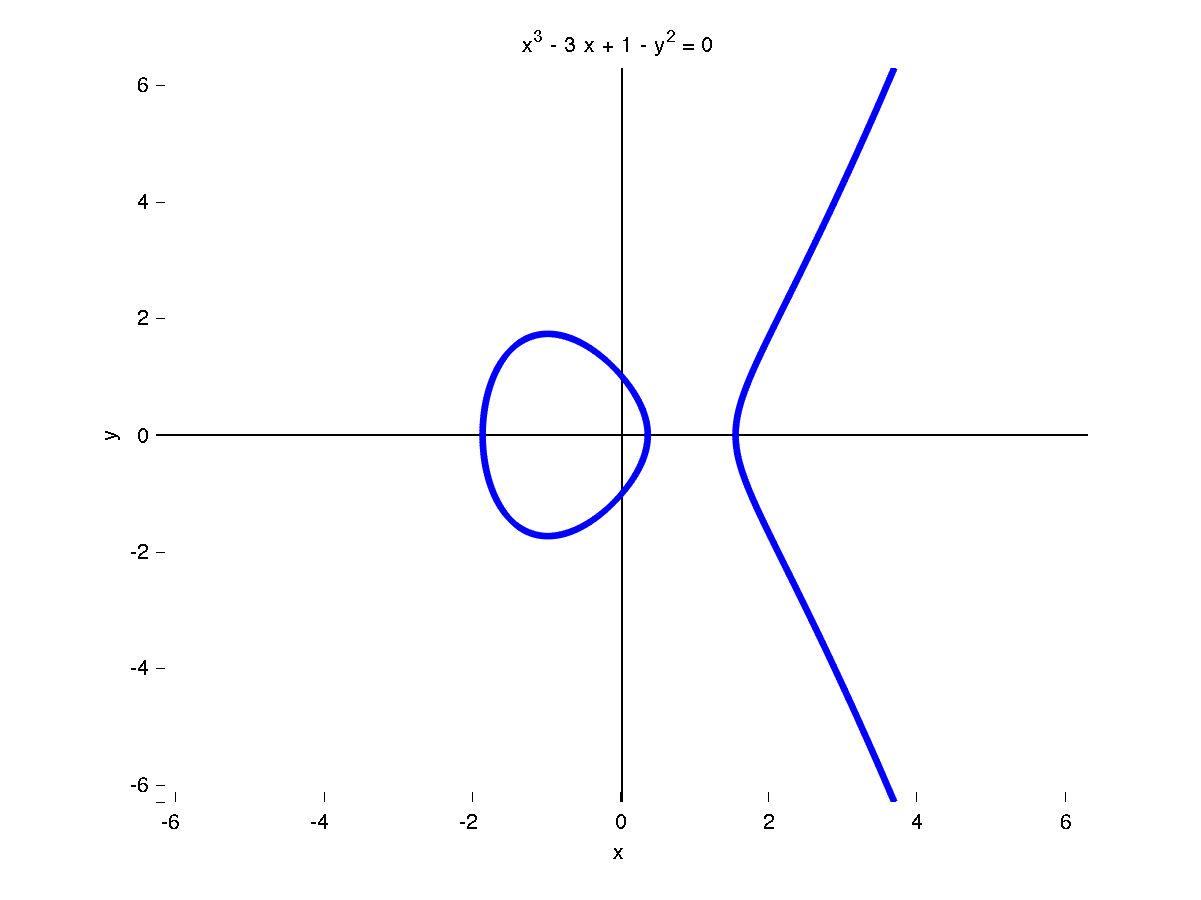
\includegraphics[width=.7\textwidth]{images/ec1.png}
\caption{The elliptic curve $y^2 = x^3 - 3x + 1$.}
\label{fig:ec-plot}
\end{figure}

Figure \ref{fig:ec-singular} shows two singular curves.
To define a group operation on the points of the curve, we need to be able to take a tangent line to each point.
So we avoid these cases with that additional restriction on the coefficients.

\begin{figure}[h]
\centering

\begin{subfigure}{.5\textwidth}
	\centering
	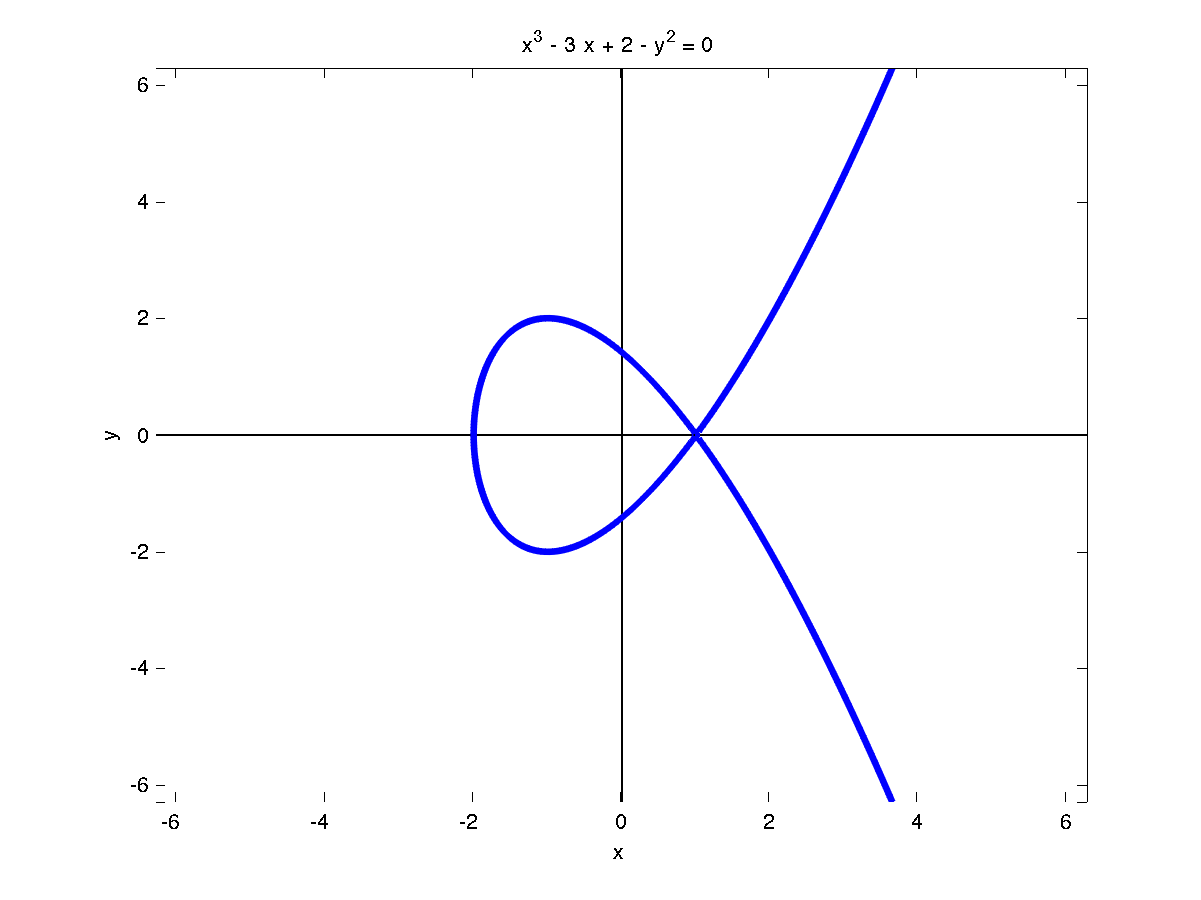
\includegraphics[width=1\linewidth]{images/ec2.png}
	\caption{The curve $y^2 = x^3 - 3x + 2$.}
\end{subfigure}%
~%
\begin{subfigure}{.5\textwidth}
	\centering
	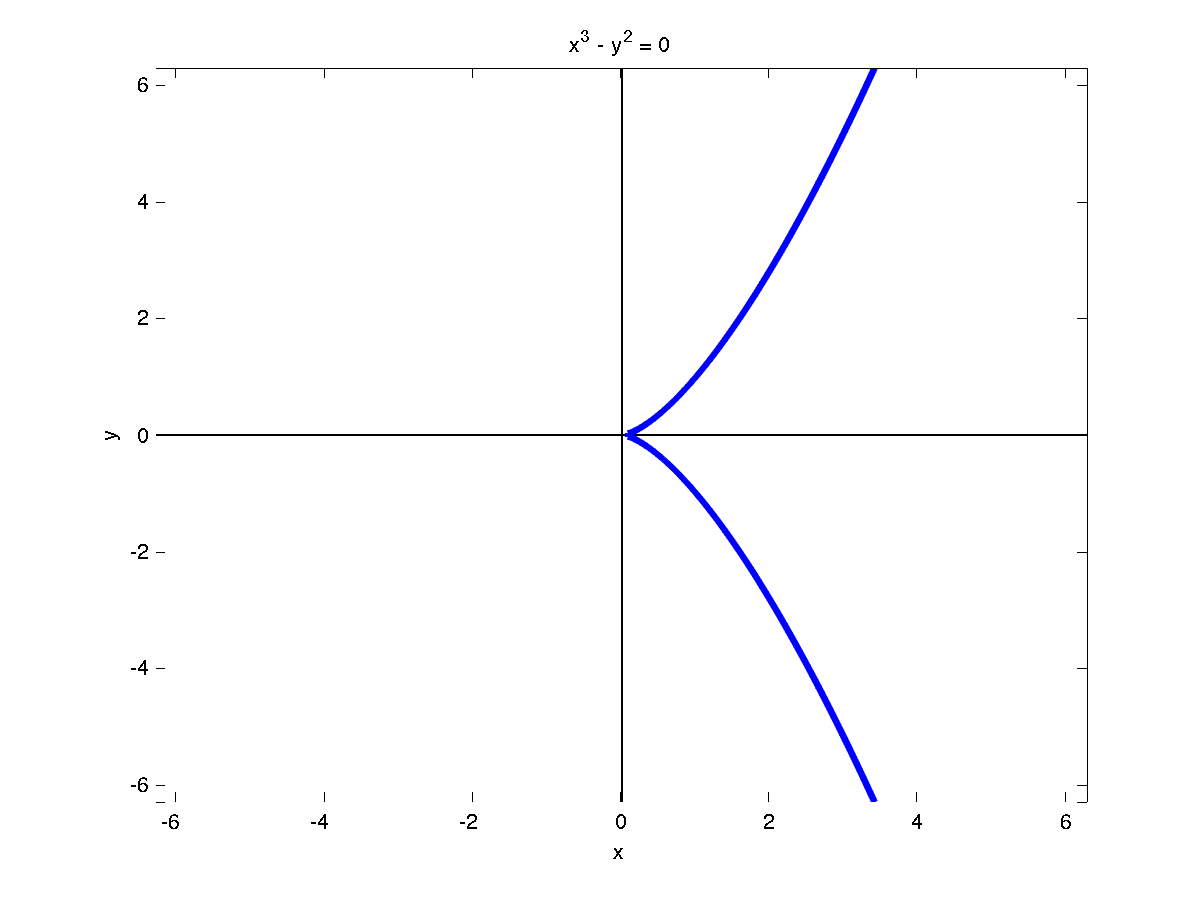
\includegraphics[width=1\linewidth]{images/ec3.png}
	\caption{The curve $y^2 = x^3$.}
\end{subfigure}

\caption{These curves have a `singularity': a point where the tangent is not clearly defined.}
\label{fig:ec-singular}
\end{figure}

\subsection{Defining a Group Operation}

\subsection{Weierstrass Form and Acceptable Changes of Variables}

\section{The Discrete Logarithm Problem}

\subsection{Trap-Door Functions}

\subsection{Attacks on Discrete Logarithms}

\section{Elliptic-Curve Diffie-Hellman Exchange}

\subsection{The Diffie-Hellman Key Exchange}

\subsection{Implementation Details of ECDH}

\begin{thebibliography}{9}

\bibitem{ecc-guide}
	Darrel Hankerson, Alfred J. Menezes, and Scott Vanstone,
	\emph{Guide to Elliptic Curve Cryptography},
	Springer,
	2004.

\bibitem{washington}
	Lawrence Washington,
	\emph{Elliptic Curves: Number Theory and Cryptography},
	Chapman and Hall/CRC,
	2nd edition,
	2008.

%\bibitem{lamport94}
%  Leslie Lamport,
%  \emph{\LaTeX: a document preparation system},
%  Addison Wesley, Massachusetts,
%  2nd edition,
%  1994.
%\cite{lamport94}

\end{thebibliography}

\end{document}